%%%%%%%%%%%%%%%%%%%%%%%%%%%%%%%%%%%%%%%%%%%%%%%%%%%%%%%%%%%%%%%%%%%
%%% Documento LaTeX 																						%%%
%%%%%%%%%%%%%%%%%%%%%%%%%%%%%%%%%%%%%%%%%%%%%%%%%%%%%%%%%%%%%%%%%%%
% Título:		Capítulo 1
% Autor:  	Ignacio Moreno Doblas
% Fecha:  	2014-02-01, actualizado 2019-11-11
% Versión:	0.5.0
%%%%%%%%%%%%%%%%%%%%%%%%%%%%%%%%%%%%%%%%%%%%%%%%%%%%%%%%%%%%%%%%%%%
% !TEX root = A0.MiTFG.tex
\chapterbegin{Propagación de pulsos ópticos ultracortos}\label{chp:ManLaTeX}
\minitoc

\begin{sinopsis}\label{sec:chpltx:sinop}
En este capítulo se analiza cuantitativamente el efecto combinado de la dispersión cromática y la turbulencia en la propagación de pulsos ópticos ultracortos a través de la atmósfera y del océano. Para ello, se desarrolla en serie de Taylor el índice de refracción del aire y del agua, obteniendo los coeficientes de dispersión $\beta_2$ y $\beta_3$ y las longitudes de dispersión asociadas. A continuación, se integra esta descripción dispersiva en el marco estadístico basado en la función de coherencia mutua y la irradiancia promedio, lo que permite derivar expresiones cerradas para el ensanchamiento temporal del pulso y definir el factor de ensanchamiento que cuantifica de forma unificada la contribución conjunta de la dispersión cromática y la turbulencia en ambos medios. 
\end{sinopsis}

%\section{Análisis del efecto de dispersión cromática}
%%%%%%%%%%%%%%%%%%%%%%%%%%%%%%%%%%%%%%%%%%%%%%%%%%%%%%%%%%%%%%%%%%%%%%%%%%%%%%%%%%%%%%%%%%%%%%%%%%%%%%%%%%%%%%%%%%%%%%%%%%%%%%%%%%%%%%
\section{Fundamentos físicos de la propagación óptica}
La propagación de un pulso óptico a través de un medio lineal dispersivo puede describirse a partir de las ecuaciones de Maxwell, dando lugar a la conocida ecuación de Helmholtz. La ecuación de Helmholtz aparece con frecuencia en el estudio de problemas físicos que involucran ecuaciones en derivadas parciales en el espacio y en el tiempo. Esta ecuación, que representa una forma independiente del tiempo de la ecuación de onda, se obtiene al aplicar la técnica de separación de variables para reducir la complejidad del análisis. Esta ecuación constituye una forma particular de la ecuación de onda y permite obtener el campo eléctrico, $\bar{E}$, aunque de manera análoga puede derivarse para el campo magnético, $\bar{H}$. Su relevancia radica en que aparece de forma recurrente en problemas de electromagnetismo y en otras áreas de la física, como la acústica o la mecánica cuántica. En el caso de la óptica, la ecuación de Helmholtz representa el punto de partida para analizar cómo se modifican las ondas al propagarse en medios con dispersión y constituye la base electromagnética para el estudio que aquí se presenta.

Por tanto, el análisis de la propagación de un pulso óptico en un medio lineal dispersivo se realiza a partir de la solución de la ecuación de Helmholtz en el dominio de la frecuencia, la cual se expresa como:
\begin{equation}
\nabla^{2}E(z,\omega)+\beta(\omega)^{2}E(z,\omega)=0.
\end{equation}
En otras palabras, se trata de la ecuación de onda en el dominio espectral para un medio lineal dispersivo con una relación de dispersión arbitraria $\beta(\omega)=\omega n(\omega)/c$ y con $\mu=1$, donde $\mu$ es la permeabilidad relativa del medio \cite{Agrawal,Keller}.

El reto consiste ahora en modelar $\beta(\omega)$ de manera que represente fielmente el comportamiento de la atmósfera terrestre como medio no guiado en el cual se propagan los pulsos ultracortos que aquí se analizan. Una vez caracterizada la atmósfera como un medio lineal cuya constante de fase depende de la frecuencia, esta ecuación se resolverá mediante simulaciones en Matlab, con el fin de estudiar la evolución del pulso a lo largo del enlace en secciones posteriores.

Cuando una onda electromagnética interactúa con los electrones presentes en un medio dieléctrico, la respuesta del medio, en general, depende de la frecuencia óptica $\omega$. Esta propiedad, denominada dispersión cromática, se manifiesta a través de la dependencia del índice de refracción con la frecuencia, tal como se ha visto anteriormente.

En sistemas de comunicaciones ópticas basados en fibra óptica, la dispersión de la fibra es crítica en la propagación de pulsos ópticos ultracortos porque diferentes componentes espectrales asociadas con el pulso viajan a diferentes velocidades dadas por $c/n(\omega)$. Incluso cuando los efectos no lineales no son importantes, el ensanchamiento del pulso inducido por la dispersión puede ser perjudicial para los sistemas de comunicaciones ópticas. En el régimen no lineal, la combinación de dispersión y no linealidad puede dar como resultado un comportamiento cualitativamente diferente. No obstante, el comportamiento no lineal derivado de la propagación de pulsos con altísima relación \acs{PAOPR}~(\acl{PAOPR}) y reducido ciclo de trabajo se escapa del objetivo del presente Trabajo Fin de Grado.

En términos matemáticos, los efectos de la dispersión cromática se estudian mediante el desarrollo en serie de Taylor de la constante de propagación $\beta(\omega)$ alrededor de la frecuencia $\omega_{0}$, en torno a la cual se encuentra centrado el espectro del pulso. Para ello se asume la aproximación de envolvente lentamente variable, de modo que:

\begin{equation}
\beta(\omega)=\dfrac{\omega\\n(\omega)}{c}\simeq 
\beta_{0} + \beta_{1}(\omega-\omega_{0}) + \dfrac{\beta_{2}}{2}(\omega-\omega_{0})^2
+ \dfrac{\beta_{3}}{6}(\omega-\omega_{0})^3+\dots
\end{equation}

donde
\begin{equation}
\beta_{k}=\left.\frac{d^{k}\beta}{d\omega^{k}}\right\vert_{\omega_{0}}.
\end{equation}
La envolvente de un pulso óptico se propaga a la velocidad de grupo $v_\mathrm{g}=1/\beta_{1}$, mientras que el parámetro $\beta_{2}$ caracteriza la dispersión de velocidad de grupo y es responsable del ensanchamiento del pulso, además de inducir cierto \textit{chirp}. Este fenómeno se conoce como dispersión de velocidad de grupo, siendo $\beta_{2}$ el denominado parámetro GVD. Por su parte, $\beta_{3}$ se conoce como parámetro TOD. Los efectos de dispersión de órdenes superiores pueden distorsionar pulsos ópticos ultracortos tanto en el régimen lineal como en el no lineal.

%%%%%%%%%%%%%%%%%%%%%%%%%%%%%%%%%%%%%%%%%%%%%%%%%%%%%%%%%%%%%%%%%%%%%%%%%%%%%%%%%%%%%%%%%%%%%%%%%%%%%%%%%%%%%%%%%%%%%%%%%%%%%%%%%%%%%%
\section{Estudio de propagación a través de la atmósfera terrestre}
\subsection{Índice de refracción del aire}
Considerando el medio en cuestión, la atmósfera terrestre, el índice de refracción puede expresarse en función de la longitud de onda $\lambda$ en m, tal como se indica en \cite{Owens,Andrews}, de la siguiente manera:
\begin{equation}\label{refractiveIndexLambda}
n(\lambda)=1+77.6\times10^{-6}\left(1+7.52\times10^{-15}\lambda^{-2}\right)\frac{P(h)}{T(h)},
\end{equation}
donde $T(h)=288.19-6.49\times10^{-3}h$ es la temperatura medida en K, $P(h)=2.23\times10^{-6}(44.41-h\times10^{-3})^{5.256}$ es la presión medida en mbar, y $h$ es la altura del enlace en m. Sin pérdida de generalidad, resulta conveniente también expresar la \mbox{Ecuación (\ref{refractiveIndexLambda})} en función de $\omega$ como:
\begin{equation}
n(\omega)=1+\frac{aP(h)}{T(h)}\left(1+\frac{b\omega^{2}}{4\pi^{2}c^{2}}\right),
\end{equation}
donde los parámetros $a$ y $b$ se definen como $a=77.6\times10^{-6}$ y $b=7.52\times10^{-15}$.

\subsubsection{Dependencia de presión, temperatura y longitud de onda}
En esta sección se analiza la dependencia del índice de refracción de la atmósfera terrestre con la longitud de onda, considerando una altura de referencia de \mbox{$h=500$ m}. La \mbox{Figura \ref{nLambda}} muestra cómo varía $n(\lambda)$ en función de la longitud de onda.
\begin{figure}[!h]
\centering
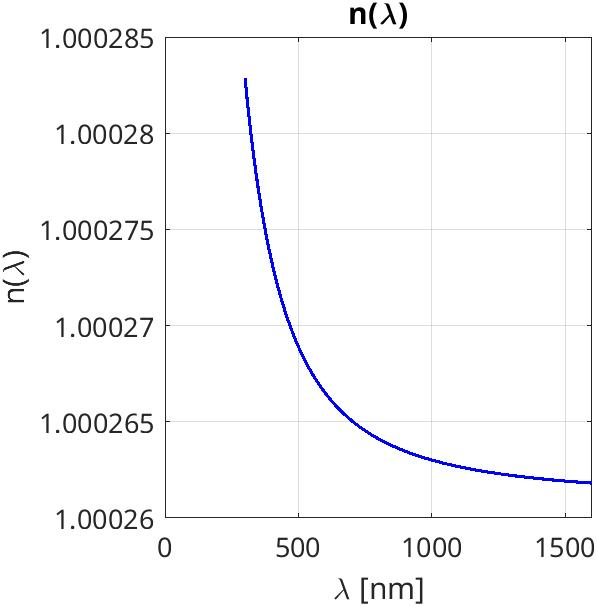
\includegraphics[scale=0.4]{./figuras/fig/nLambda.jpg}
\caption{Representación del índice de refracción de la atmósfera terrestre para una altura de \mbox{$h=500$ m} en función de la longitud de onda}
\label{nLambda}
\end{figure}

Se observa que el índice de refracción disminuye ligeramente al aumentar la longitud de onda, reflejando la dispersión cromática natural del aire. Aunque la variación es pequeña, esta dependencia es la que da lugar al ensanchamiento de los pulsos a medida que se propagan a través del medio.

Dado que las variaciones de $n(\lambda)$ con la longitud de onda son relativamente leves, surge una pregunta abierta: ¿cuánto impacto tendrá esta dispersión sobre el ensanchamiento de los pulsos en función de la duración y forma de los mismos? Esta cuestión se abordará en secciones posteriores mediante simulaciones numéricas que permiten evaluar de forma cuantitativa la influencia de la atmósfera sobre pulsos ultracortos.

Antes de continuar, y con el objetivo de ofrecer una representación visual de la evolución de los parámetros más relevantes de la atmósfera terrestre, en particular el índice de refracción, la temperatura y la presión, en la \mbox{Figura \ref{indiceCompleto}} se muestran gráficos que ilustran cómo varían dichos parámetros en función de la altura del enlace.
\begin{figure}[!h]
\centering
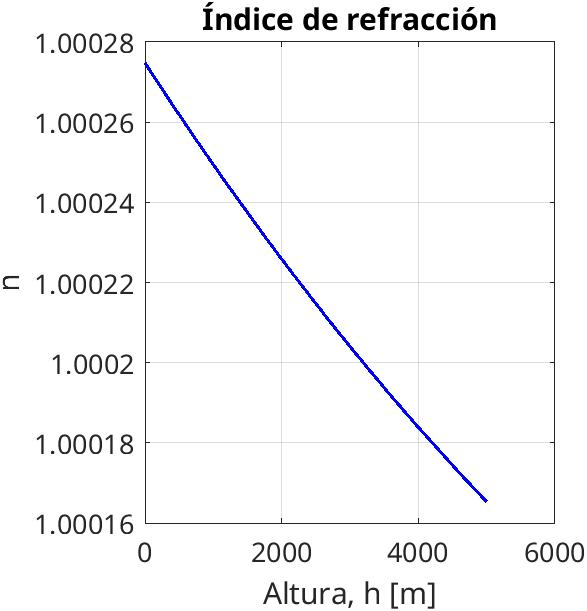
\includegraphics[scale=0.23]{./figuras/fig/nAT.jpg}
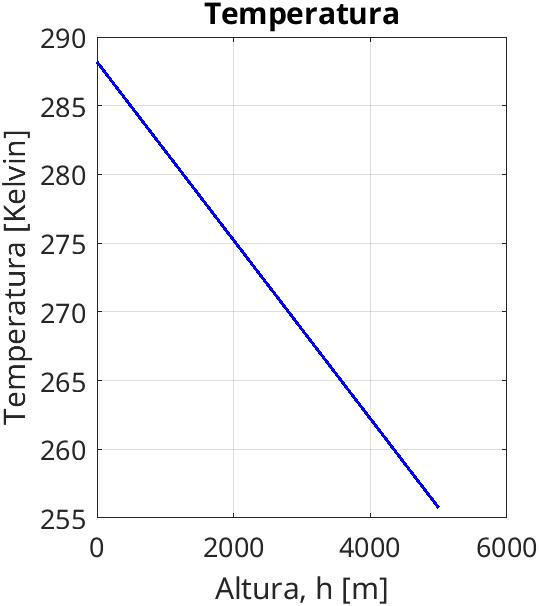
\includegraphics[scale=0.23]{./figuras/fig/tAT.jpg}
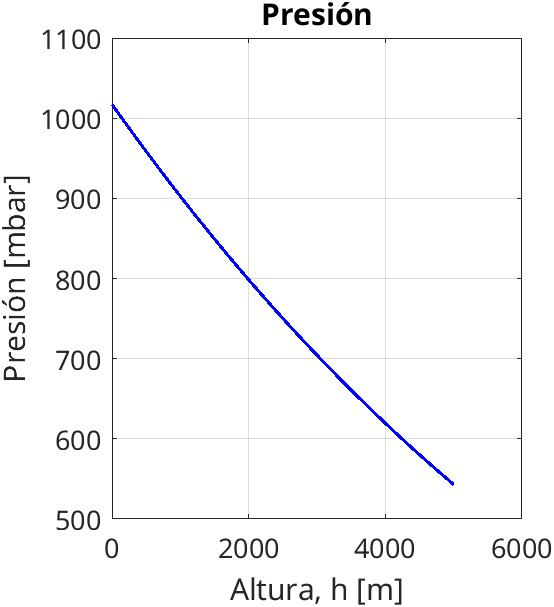
\includegraphics[scale=0.23]{./figuras/fig/pAT.jpg}
\caption{Representación del índice de refracción de la atmósfera terrestre para \mbox{$\lambda=1550$ nm}, la temperatura, $T(h)$, y la presión, $P(h)$, en función de la altura del enlace $h$ en metros}
\label{indiceCompleto}
\end{figure}

En ellos se puede observar que, a medida que se incrementa la altitud, tanto la temperatura como la presión y, por consiguiente, el índice de refracción, presentan un comportamiento decreciente, reflejando la disminución de la densidad atmosférica en capas superiores. Esta representación facilita la comprensión del impacto de las condiciones atmosféricas sobre la propagación de pulsos ópticos ultracortos en enlaces FSO terrestres.

\subsection{Análisis de la dispersión cromática}
Con el fin de expresar el índice de refracción del aire mediante un desarrollo en serie de Taylor, se simplifica previamente su expresión, agrupando el término  $a\,P(h)/T(h)$ en una constante que se denota por $K$. Sustituyendo esta definición en la expresión del índice de refracción del aire y reorganizando los términos, se obtiene una forma más compacta que facilita los cálculos posteriores:
\begin{equation}
\begin{gathered}
n(\omega)
= 1 + K\left(1 + \frac{b\,\omega^{2}}{4\pi^{2}c^{2}}\right)
= (1+K) + \frac{K b}{4\pi^{2}c^{2}}\,\omega^{2}
\equiv C_{1} + C_{2}\,\omega^{2},\\[4pt]
C_{1} = 1+K,\qquad
C_{2} = \frac{K b}{4\pi^{2}c^{2}}.
\end{gathered}
\end{equation}
De este modo, el índice de refracción queda expresado directamente como un polinomio cuadrático en $\omega$, lo que permite aplicar de manera inmediata el desarrollo en serie de Taylor en torno a la frecuencia angular $\omega_0$. Al tratarse de una función polinómica de segundo grado, las derivadas de orden superior se anulan. La forma general del desarrollo es, por tanto:
\begin{equation}
n(\omega) = n(\omega_0) + \left. \frac{d n}{d \omega} \right|_{\omega_0} (\omega - \omega_0) 
+ \frac{1}{2} \left. \frac{d^2 n}{d \omega^2} \right|_{\omega_0} (\omega - \omega_0)^2.
\end{equation}
Si se particuliza para la expresión del índice de refracción considerada, las derivadas correspondientes son:

\begin{equation}
\begin{aligned}
n(\omega_0) &= \mathcal{C}_1 + \mathcal{C}_2\,\omega_0^2 \equiv n_0,\\
\left. \frac{d n}{d \omega} \right|_{\omega_0} &= 2\,\mathcal{C}_2\,\omega_0 \equiv n_1,\\
\left. \frac{d^2 n}{d \omega^2} \right|_{\omega_0} &= 2\,\mathcal{C}_2 \equiv n_2,\\
\left. \frac{d^3 n}{d \omega^3} \right|_{\omega_0} &= 0.
\end{aligned}
\end{equation}


donde $n_0$, $n_1$ y $n_2$ representan, respectivamente, los coeficientes del desarrollo en serie de Taylor asociados al valor del índice de refracción y a sus derivadas primera y segunda en torno a $\omega_0$.


A partir de estas derivadas, la expansión en serie de Taylor puede escribirse como:
\begin{equation}
n(\omega) \approx \mathcal{C}_1 + \mathcal{C}_2 {\omega_0}^2 
+ 2\mathcal{C}_2 \omega_0 (\omega - \omega_0) 
+ \mathcal{C}_2 (\omega - \omega_0)^2.
\end{equation}
Dado que la constante de propagación se define como $\beta(\omega) = \omega\,n(\omega)/c$, un desarrollo en serie de Taylor del índice de refracción conduce de forma directa a un desarrollo equivalente de la constante de propagación. El desarrollo en serie de Taylor de la constante de propagación centrado en $\omega_0$ tiene la forma general:
\begin{equation}
\beta(\omega) \approx \beta_0 + \beta_1 (\omega - \omega_0) + \frac{\beta_2}{2} (\omega - \omega_0)^2 + \frac{\beta_3}{6} (\omega - \omega_0)^3 + \dotsb
\end{equation}
Cada término de esta serie se obtiene derivando la expresión general de la constante de propagación, como:
\begin{equation}
\begin{split}
&\beta_0 = \beta(\omega_0) = \frac{\omega_0\,n(\omega_0)}{c},\\
&\beta_1 = \left. \frac{d\beta}{d\omega} \right|_{\omega_0}
         = \frac{1}{c}\left[ n(\omega_0) + \omega_0\,n'(\omega_0) \right], \\ \\
&\beta_2 = \left. \frac{d^2 \beta}{d\omega^2} \right|_{\omega_0}
         = \frac{1}{c}\left[ 2\,n'(\omega_0) + \omega_0\,n''(\omega_0) \right],\\
&\beta_3 = \left. \frac{d^3 \beta}{d\omega^3} \right|_{\omega_0}
         = \frac{1}{c}\left[ 3\,n''(\omega_0) + \omega_0\,n'''(\omega_0) \right].
\label{eq:beta3}
\end{split}
\end{equation}
donde $\beta_0$, $\beta_1$, $\beta_2$ y $\beta_3$ representan los coeficientes del desarrollo en serie de Taylor de la constante de propagación, correspondientes respectivamente al valor de $\beta(\omega)$ y a sus derivadas primera, segunda y tercera en torno a $\omega_0$.

Usando las abreviaturas $n_0$, $n_1$, $n_2$ y $n_3$ , con $n_0 = n(\omega_0)$, $n_1 = n'(\omega_0)$, $n_2 = n''(\omega_0)$ y $n_3 = n'''(\omega_0)$, se tiene:

\begin{equation}
\begin{split}
&\beta_0 = \frac{\omega_0\,n_0}{c},\\
&\beta_1 = \frac{n_0 + \omega_0\,n_1}{c},\\ 
&\beta_2 = \frac{2\,n_1 + \omega_0\,n_2}{c},\\
&\beta_3 = \frac{3\,n_2 + \omega_0\,n_3}{c}.
\end{split}
\end{equation}

A continuación, en la \mbox{Figura \ref{betaWVL}}, se muestra la constante de fase $\beta(\omega)$ en función de la longitud de onda $\lambda$ para una altura de referencia de \mbox{$h=500$ m}, destacando un comportamiento decreciente con la longitud de onda, y en la \mbox{Figura \ref{GVDTOD}}, se representan los parámetros $\beta_{2}$ y $\beta_{3}$, evidenciando el comportamiento decreciente de ambos con la altura.
\begin{figure}[!h]
\centering
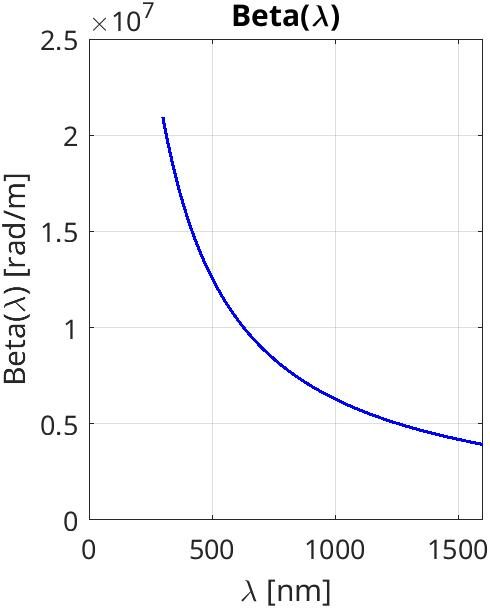
\includegraphics[scale=0.4]{./figuras/fig/beta.jpg}
\caption{Representación de la constante de fase, $\beta(\lambda)$, en función de $\lambda$ para una altura de referencia de \mbox{$h=500$ m}}
\label{betaWVL}
\end{figure}

Estos resultados están en consonancia con los observados respecto a la dependencia del índice de refracción de la atmósfera terrestre con la longitud de onda.

Con el fin de extraer conclusiones más precisas, se procede ahora a analizar los parámetros de segundo y tercer orden del desarrollo en serie de Taylor de la constante de fase, como se muestra en la \mbox{Figura \ref{GVDTOD}}.
\begin{figure}[!h]
\centering
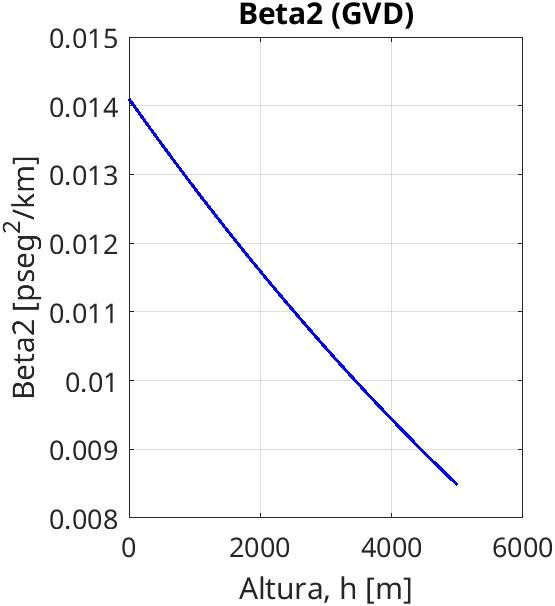
\includegraphics[scale=0.3]{./figuras/fig/beta2.jpg}
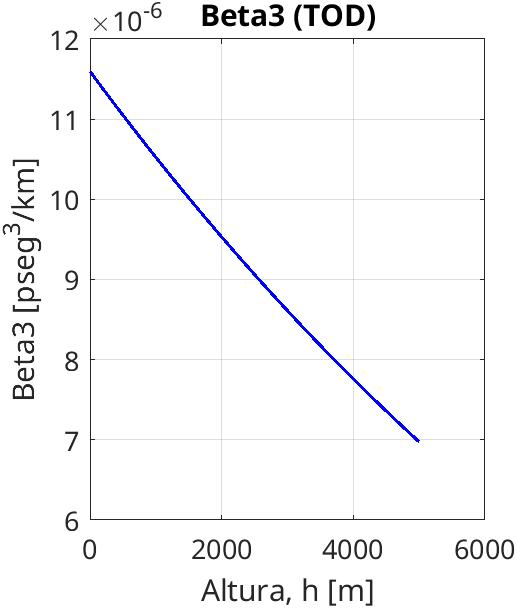
\includegraphics[scale=0.3]{./figuras/fig/beta3.jpg}
\caption{Representación de $\beta_{2}$ y $\beta_{3}$ para \mbox{$\lambda=1550$ nm} en función de la altura del enlace $h$ en metros}
\label{GVDTOD}
\end{figure}

A la vista de los resultados, se observa que $\beta_{2}$, responsable del ensanchamiento de los pulsos, tendrá un impacto limitado siempre que estos no sean extremadamente estrechos en el dominio temporal. Este comportamiento se refleja en la longitud de dispersión asociada,
\begin{equation}
L_{D}=\frac{2\sigma_{0}^{2}}{|\beta_{2}|}\approx1\text{ km},
\end{equation}
para un pulso con $FWHM=2.35,\sigma_{0}\approx 0.2$ pseg, \mbox{$\beta_2=0.0135$ pseg$^{2}$/km}, y una altura de referencia de $h=500$ m. Aquí, $\sigma_{0}=FWHM/2\sqrt{2\ln2}$ representa la anchura RMS inicial del pulso gaussiano (se adopta esta forma gaussiana por simplicidad en el análisis), mientras que FWHM denota el \textit{Full Width at Half Maximum}. Nótese además que la anchura RMS se relaciona con el parámetro temporal $T_{0}$ mediante $\sigma_{0}=T_{0}/\sqrt{2}$. En consecuencia, esto sugiere que la dispersión de segundo orden comienza a ser relevante únicamente en enlaces con longitudes del orden del kilómetro o superiores cuando se emplean pulsos con anchura temporal inferior al picosegundo.

Por otro lado, $\beta_{3}$, asociado a la dispersión de tercer orden (TOD), suele tener un efecto aún más reducido, llegando a ser despreciable en muchas condiciones prácticas. Este comportamiento queda reflejado en la longitud de dispersión de tercer orden,
\begin{equation}
L_{D}^{\prime}=\frac{\left(\sqrt{2}\sigma_{0}\right)^{3}}{|\beta_{3}|}\approx157\text{ km},
\end{equation}
para los mismos parámetros de pulso y altura y \mbox{$\beta_3=1.105\times 10^{-5}$ pseg$^{3}$/km}, lo que sugiere que los efectos de TOD sólo se vuelven relevantes en enlaces extremadamente largos o para pulsos ultracortos de anchura aún menor.

Se puede concluir, por tanto, que la relevancia de $\beta_{2}$ y $\beta_{3}$ dependerá del escenario de aplicación, de las características del láser pulsado, de la distancia del enlace y del régimen de dispersión predominante, pudiendo considerarse $\beta_{3}$ despreciable en enlaces terrestres de longitud típica.

Esta representación proporciona una visión práctica de cómo los distintos órdenes de dispersión afectan a la propagación de pulsos ópticos ultracortos a través de la atmósfera terrestre, facilitando la estimación de su influencia en sistemas de comunicaciones ópticas o experimentos de sistemas FSO.

%\subsection{Simulación Numérica de Pulsos Ultracortos}

%\subsubsection{Implementacion de la NLSE}

%\subsubsection{Resultados de simulación en Matlab}

%\subsubsection{Ensanchamiento, chirp y efecto de $\beta_2$, $\beta_3$}

%%%%%%%%%%%%%%%%%%%%%%%%%%%%%%%%%%%%%%%%%%%%%%%%%%%%%%%%%%%%%%%%%%%%%%%%%%%%%%%%%%%%%%%%%%%
\subsection{Efecto de la turbulencia atmosférica}

\subsubsection{Motivación del análisis}
Comprender los mecanismos que degradan los pulsos ópticos resulta esencial para el diseño de sistemas de comunicación óptica fiables, tal y como se comentó anteriormente en esta memoria. Entre estos efectos destacan principalmente el ensanchamiento temporal del pulso, cuyo análisis se basa en la función de coherencia mutua.

El interés por este campo ha crecido en las últimas décadas, especialmente en el contexto de pulsos ultracortos. Los pulsos en el régimen de fseg exigen un tratamiento en el dominio de la frecuencia, aumentando la complejidad de su análisis. Hasta ahora, los efectos de la turbulencia atmosférica y de la dispersión cromática han sido estudiados de forma separada en la propagación de pulsos ópticos ultracortos. En este trabajo, sin embargo, y bajo la aproximación de campo cercano como primera aproximación al análisis, se presentan resultados de ensanchamiento temporal considerando simultáneamente ambos efectos. De este modo, se avanza más allá de los estudios previos que, en su mayoría, se han centrado en la evolución temporal de pulsos gaussianos en espacio libre y en la cuantificación del ensanchamiento de forma independiente. Aunque existen soluciones analíticas en casos particulares, como los modelos de la MCF para ondas planas o haces gaussianos en regímenes de turbulencia débil, la mayor parte de los estudios disponibles se han apoyado en aproximaciones numéricas \cite{Andrews} (y sus referencias).

\subsubsection{MCF}
En los últimos años ha surgido un gran interés en el estudio de la propagación de pulsos ópticos a través de la atmósfera. Este interés se debe al amplio ancho de banda disponible a frecuencias elevadas, que abre la puerta a comunicaciones por pulsos con altas tasas de transmisión de datos. Por razones de simplicidad matemática, la mayoría de los estudios teóricos se han centrado en ondas planas ilimitadas o esféricas. Sin embargo, en \cite{Young1996}, se analiza el pulso de haz gaussiano, que representa de manera más realista un haz láser real, y sentando las bases de este análisis, incorporando el efecto de la dispersión cromática.

Las características de propagación de un pulso en un medio aleatorio vienen determinadas por la MCF, que se define como:
\begin{equation}
\Gamma_2(\mathbf{r}_1, k_1, \mathbf{r}_2, k_2, z) = \langle U(\mathbf{r}_1, k_1, z)\, U^*(\mathbf{r}_2, k_2, z) \rangle,
\end{equation}
donde $\langle \cdot \rangle$ representa un promedio estadístico, $U(\mathbf{r}, k, z)$ es el campo óptico, $\mathbf{r}$ es un vector en el plano transversal a la distancia de propagación $z$, y $k$ es el número de onda en el punto $(\mathbf{r}, z)$. A partir de esta MCF es posible deducir las principales propiedades estadísticas del pulso, tales como el ensanchamiento temporal, entre otros. Utilizando la aproximación de Rytov de primer orden, se define el campo óptico a una distancia de propagación $z$ como:
\begin{equation}
U(\mathbf{r}, k, z) = U_{0}(\mathbf{r}, k, z) \exp \left[ \Psi(\mathbf{r}, k, z) \right],
\end{equation}
donde $U_{0}(\mathbf{r}, k, z)$ es el campo en ausencia de inhomogeneidades aleatorias, y $\Psi(\mathbf{r}, k, z)$ representa las perturbaciones de fase complejas de primer orden causadas por dichas inhomogeneidades.

El análisis desarrollado en este trabajo se enmarca dentro de la aproximación de campo cercano para un haz gaussiano, es decir, en el régimen en el que la distancia de propagación es corta en comparación con la longitud de Rayleigh y el haz conserva un radio próximo al de su cintura. Si bien este estudio deberá extenderse en el futuro al campo lejano, cabe destacar que, cuando se considera únicamente el efecto de la turbulencia atmosférica en el ensanchamiento de los pulsos ultracortos, los resultados obtenidos coinciden con los que se esperan en dicho régimen \cite{Andrews}. Por ello, no resulta aventurado anticipar, aunque deba confirmarse en trabajos futuros, que las conclusiones aquí presentadas podrían ser también válidas en el campo lejano.

Por último, es importante destacar que el desarrollo completo de la MCF implica una complejidad matemática considerable, que puede abordarse en detalle en referencias especializadas, como en \cite{Andrews}. Dado que en este trabajo la MCF se utiliza principalmente como herramienta dentro del análisis de propagación de pulsos, se limita aquí a una presentación introductoria, suficiente para comprender su papel y su aplicación en los resultados posteriores.

\subsubsection{Análisis de la dispersión temporal}
Consideremos un pulso de entrada en el plano del transmisor ($z=0$) que se propaga a través de un medio aleatorio hasta un receptor ubicado a una distancia $z$ del transmisor. Se toma el caso en el que el pulso de entrada es una señal modulada sobre una frecuencia portadora angular $\omega_{0}$. Tomando como referencia el campo eléctrico, el campo a la salida del sistema, entendiendo sistema como el conjunto formado por transmisor, canal y receptor, puede representarse como:
\begin{equation}
E_{out}(z,t)=e^{\mathrm{j}\omega_{0}t}\int_{-\infty}^{+\infty}F(\omega)H(\mathrm{j}\left(\omega+\omega_{0}\right))e^{\mathrm{j}\omega t}d\omega,
\end{equation}
donde $F(\omega)$ es la transformada de Fourier del pulso en $z=0$, $H(\mathrm{j}\omega)=e^{-j\beta(\omega)z}=e^{-j\frac{\omega n(\omega)}{c}z}$ es la respuesta en frecuencia del medio, considerando únicamente los efectos de fase y obviando, como se hizo anteriormente, las pérdidas. Esta respuesta puede expresarse de forma más general considerando los efectos aleatorios de la atmósfera:
\begin{equation}
H(j\omega)=U_{0}(r,z;\omega)e^{\Psi\left(r,z;\omega\right)},
\end{equation}
donde $U_{0}(r,z;\omega)=V(r,z)e^{-\mathrm{j}\beta(\omega)z}$, $V(r,z)$ representa una variación espacial asociada a una onda de haz gaussiano \cite{Andrews}, y $\Psi\left(r,z;\omega\right)$ corresponde a la perturbación de fase inducida por la turbulencia atmosférica. Finalmente, tras las correspondientes manipulaciones algebraicas, la expresión que debe resolverse queda determinada por:
\begin{equation}
E_{out}(r,z;t)=e^{\mathrm{j}\omega_{0}t}\int_{-\infty}^{+\infty}F(\omega)\left[V(r,z)e^{-\mathrm{j}\beta\left(\omega+\omega_{0}\right)z}e^{\Psi\left(r,z;\omega+\omega_{0}\right)}\right]e^{\mathrm{j}\omega t}d\omega,
\end{equation}
Asumiendo un perfil gaussiano tanto en el plano espacial como en el temporal, se analiza el ensanchamiento temporal del pulso debido no solo a la dispersión cromática, sino también al efecto de la turbulencia atmosférica. Bajo estas condiciones, la forma temporal del pulso gaussiano se expresa como:
\begin{equation}
f(t)\propto e^{-\frac{t^{2}}{2\sigma_{0}}},
\end{equation}
donde $\sigma_0$ representa la anchura temporal RMS. Aunque los pulsos muy cortos, del orden de los fseg, suelen clasificarse como de banda ancha, la forma de onda transmitida puede aún considerarse de banda estrecha si $\Delta \omega \ll \omega_0$, donde $\omega_0$ es la frecuencia portadora óptica.

El ensanchado temporal del pulso en un medio aleatorio es debido, principalmente, al proceso de \textit{scattering} del medio (dispersión producida por los diferentes caminos), y al efecto de \textit{wandering} del pulso. Este último es dominante en régimen de fluctuaciones débiles. El efecto combinado de ambos mecanismos de ensanchado se deduce a partir de la irradiancia media del pulso obtenido a partir de la MCF, que se define como:
\begin{equation}
\begin{split}
&<I(r,z;t)>=\frac{\sigma_{0}^{2}}{\pi}\int_{-\infty}^{+\infty}\int_{-\infty}^{+\infty}e^{-2\sigma_{0}^{2}\omega_{c}^{2}}e^{-\frac{\sigma_{0}^{2}}{2}\omega_{d}^{2}}\\
&\times\Gamma_{2}\left(r,r,z;\omega_{0}+\omega_{c}+\frac{1}{2}\omega_{d},\omega_{0}+\omega_{c}-\frac{1}{2}\omega_{d}\right)e^{j\omega_{d}t}d\omega_{c}d\omega_{d},
\end{split}
\end{equation}
donde $\Gamma_2(\cdot)$ es la MCF, $\omega_{c}=\frac{1}{2}\left(\omega_{1}+\omega_{2}\right)$ y $\omega_{d}=\left(\omega_{1}-\omega_{2}\right)$. Tal como se mencionó en la subsección anterior, y con el fin de obtener expresiones matemáticas en forma cerrada que permitan analizar el impacto de las distintas fuentes de ensanchamiento,se recurre inicialmente a la aproximación de campo cercano. Bajo esta aproximación, válida en el contexto de nuestro estudio, la MCF $\Gamma_2(\cdot)$ de la expresión anterior puede aproximarse como en \cite{Andrews}, teniendo en cuenta $\beta(\omega)$, como:
\begin{equation}
\Gamma_2(\cdot)=e^{-\frac{2r^{2}}{W_{0}}}\times e^{-\mathrm{j}\left(\beta(\omega_{1}+\omega_{0})-\beta(\omega_{2}+\omega_{0})\right)}\times e^{-a_{T}\omega_{d}^{2}},
\end{equation}
donde el parámetro $a_{T}$, introducido aquí por primera vez, será el encargado de cuantificar la importancia del efecto turbulento de la atmósfera sobre la propagación de pulsos ultracortos. Aplicando la aproximación de banda estrecha, $\omega_{d}^{2}\ll\omega_{c}^{2}$, el parámetro $a_{T}$, que depende de la densidad espectral de potencia de las fluctuaciones del índice de refracción en la atmósfera, $\Phi(\kappa)$, puede calcularse considerando el espectro de von Kármán como:
\begin{equation}
a_{T}=\frac{2\pi^{2}z}{c^{2}}\int_{0}^{\infty}\kappa\Phi(\kappa)d\kappa\simeq\frac{0.39C_{n}^{2}z\kappa_{0}^{-5/3}}{c^{2}},
\end{equation}
donde $C_{n}^{2}$ es el parámetro de estructura del índice de refracción y representa un indicador de la fuerza de la turbulencia, y $\kappa_{0}$ está relacionado con el modelo de densidad espectral de potencia de las fluctuaciones del índice de refracción usado.

Considerando ahora la dispersión cromática hasta el término de segundo orden, $\beta_2$ (GVD), y habiendo concluido en el apartado anterior que el término de tercer orden, $\beta_3$ (TOD), puede considerarse despreciable, la expresión de la irradiancia media se obtiene tras realizar varias manipulaciones algebraicas, que se omiten aquí para no dificultar la lectura, como sigue:
\begin{equation}
\begin{split}
<I(r,z;t)>=&\frac{\sigma_{0}^{2}}{\pi}e^{-\frac{2r^{2}}{W_{0}^{2}}}\\
&\int_{-\infty}^{+\infty}e^{-2\sigma_{0}^{2}\omega_{c}^{2}}\left[\int_{-\infty}^{+\infty}e^{-\omega_{d}^{2}\left(\frac{\sigma_{0}^{2}}{2}+a_{T}\right)}e^{\mathrm{j}\omega_{d}\left(t-\beta_{1}z-\beta_{2}\omega_{c}z\right)}d\omega_{d}\right]d\omega_{c}.
\end{split}
\end{equation}
La doble integral de la expresión anterior se resuelve mediante manipulaciones algebraicas y haciendo uso de $\int_{-\infty}^{\infty}e^{-ax^2+2bx}dx=\sqrt{\frac{\pi}{a}}e^{b^2/a}$ \cite{Gradshteyn}, que se omiten aquí por simplicidad, obteniéndose finalmente la expresión de la irradiancia promedio, $<I(r,z;t)>$, como:
\begin{equation}
<I(r,z;t)>=\frac{e^{-\frac{2r^{2}}{W_{0}}}}{BF_{\text{comb}}}\times e^{-\frac{2(t-\beta_{1}z)^{2}}{4\sigma_{0}^{2}BF_{\text{comb}}^{2}}},
\end{equation}
donde $W_{0}$ es la cintura de haz, y $BF_{\text{comb}}$ es el factor de ensanchamiento, que cuantifica conjuntamente el efecto de la turbulencia atmosférica en régimen de turbulencia débil y el efecto de la dispersión cromática, y cuya expresión se obtiene como:
\begin{equation}
%BF=\sqrt{\frac{2a_{1}}{\sigma_{0}^{2}}+\left(1+\frac{C\beta_{2}z}{2\sigma_{0}^{2}}\right)^{2}+\left(\frac{\beta_{2}z}{2\sigma_{0}^{2}}\right)^{2}+\left(1+C^{2}\right)^{2}\frac{1}{2}\left(\frac{\beta_{3}z}{4\sigma_{0}^{3}}\right)^{2}},
%BF=\sqrt{\frac{2a_{T}}{\sigma_{0}^{2}}+\left(1+\frac{C\beta_{2}z}{2\sigma_{0}^{2}}\right)^{2}+\left(\frac{\beta_{2}z}{2\sigma_{0}^{2}}\right)^{2}}.
BF_{\text{comb}}=\sqrt{1+\frac{2a_{T}}{\sigma_{0}^{2}}+\left(\frac{\beta_{2}z}{2\sigma_{0}^{2}}\right)^{2}}.
\end{equation}

%\subsubsection{Factor de ensanchado}

%%%%%%%%%%%%%%%%%%%%%%%%%%%%%%%%%%%%%%%%%%%%%%%%%%%%%%%%%%%%%%%%%%%%%%%%%%%%%%%%%%%%%%%%%%%%%%%%%%%%%%%%%%%%%%%%%%%%%%%%%%%%%%%%%%%%%%
\section{Estudio de propagación a través del océano}

\subsection{Índice de refracción del agua}

Considerando ahora el medio oceánico, el índice de refracción del agua presenta una dependencia más compleja que en el caso atmosférico, ya que es necesario incorporar explícitamente parámetros adicionales como la salinidad, además de la presión, la temperatura y la longitud de onda. Ignorar estos efectos equivaldría a describir agua pura o destilada, lo que no representa de forma realista el entorno marino.

En este trabajo se emplea la formulación de Millard y Seaver \cite{Millard}, basada en un algoritmo empírico de 27 términos obtenido a partir de cuatro conjuntos experimentales distintos. Este modelo ha sido ampliamente utilizado para describir el comportamiento óptico del agua de mar y es válido para longitudes de onda comprendidas entre \SI{500}{\nano\meter} y \SI{700}{\nano\meter}, temperaturas entre \SI{0}{\celsius} y \SI{30}{\celsius}, salinidades entre \SI{0}{\psu} y \SI{40}{\psu} y presiones de hasta \SI{11000}{\deci\bar}, cubriendo así el rango típico de condiciones oceánicas.

La expresión general adoptada para el índice de refracción del agua puede escribirse como:
\begin{equation}
N(T,p,S,\lambda) = N_I(T,\lambda) + N_{II}(T,\lambda,S) + N_{III}(p,T,\lambda) + N_{IV}(S,p,T),
\label{eq:descomp_N_oceano}
\end{equation}
donde cada término representa la contribución correspondiente a los distintos conjuntos experimentales empleados en \cite{Millard}. En particular, $N_I$ describe el comportamiento del agua pura a presión atmosférica, a partir de los datos experimentales de Tilton y Talor obtenidos mediante el método del prisma de mínima desviación \cite{Tilton}. El término $N_{II}$ introduce la dependencia con la salinidad para agua de mar a salinidad estándar, usando los datos de Méhu y Johannin-Gilles, también obtenidos mediante el método del prisma de mínima desviación \cite{Mehu}. Por su parte, los términos $N_{III}$ y $N_{IV}$ recogen los efectos asociados a la presión, tanto en agua pura como en agua de mar, a partir de medidas experimentales realizadas bajo condiciones de alta presión.


Con el fin de integrar esta descripción dentro del formalismo de propagación empleado en este capítulo, resulta conveniente expresar el índice de refracción en función de la frecuencia angular $\omega$. Partiendo de la relación fundamental: \begin{equation}
\lambda = \frac{2\pi c}{\omega},
\end{equation}
y teniendo en cuenta que en la formulación original la longitud de onda se expresa en micrómetros, se define la constante $K = 2\pi c \times 10^{6}$, de modo que:
\begin{equation}
\lambda(\mu m) = \frac{K}{\omega}.
\end{equation}

Tras reescribir los términos dependientes de la longitud de onda en función de la frecuencia y agruparlos por potencias de $\omega$, el índice de refracción del agua puede expresarse de forma compacta como:
\begin{equation}
n(\omega) = C_0 + \frac{A}{\omega} + \frac{B}{\omega^2} + C\,\omega^2 + D\,\omega^4 + E\,\omega^6.
\label{eq:n_agua_compacto}
\end{equation}



\subsubsection{Dependencia de temperatura, salinidad, presión y longitud de onda}

En esta sección se analiza la dependencia de forma explícita del índice de refracción del agua con la temperatura, la salinidad, la presión y la longitud de onda. En particular, el índice de refracción presenta una dependencia inversa con la longitud de onda, de modo que su valor disminuye al aumentar $\lambda$. Este comportamiento es más acusado que en el caso atmosférico, especialmente en el rango espectral azul-verde, donde el índice de refracción alcanza valores más elevados y su variación espectral resulta más significativa \cite{Quan}.

La salinidad introduce una contribución adicional al índice de refracción que resulta esencial para describir de manera realista el entorno oceánico. Diversos estudios experimentales han demostrado que el valor del índice aumenta de manera aproximadamente lineal con la salinidad. En consecuencia, incluso pequeñas variaciones en la concentración de sales pueden producir cambios apreciables en las propiedades ópticas del medio \cite{Millard, Quan}.

Por su parte, la temperatura y la presión modulan el comportamiento óptico del agua a través de variaciones en la densidad y en las propiedades microscópicas del medio. En este sentido, la literatura científica coincide en que el índice de refracción disminuye de forma suave y sistemática al aumentar la temperatura. En cuanto a la presión, el índice de refracción aumenta con la presión hidrostática, un efecto que resulta relativamente pequeño en aguas superficiales, pero que adquiere mayor relevancia en escenarios de aguas profundas \cite{Millard, Quan}.

Con el objetivo de ilustrar de forma cuantitativa las dependencias descritas anteriormente, en la Tabla~\ref{tab:QuanTabla1} se presentan datos experimentales del índice de refracción del agua en función de la longitud de onda y la temperatura, para dos valores representativos de salinidad correspondientes a agua pura y agua de mar estándar, a presión atmosférica. Estos datos permiten observar de manera directa la disminución del índice de refracción con la longitud de onda y con la temperatura, así como el incremento del índice asociado a la salinidad, siendo sistemáticamente mayor en agua de mar que en agua pura.

\begin{table}[H]
\centering
\setlength{\tabcolsep}{6pt}
\renewcommand{\arraystretch}{1.15}
\scriptsize
\begin{tabular}{c c c c c c c c c}
\hline
$\lambda$ (nm) & $S$ (\textperthousand) & \multicolumn{7}{c}{\textbf{Temperatura ($^\circ$C)}} \\
\cline{3-9}
 &  & 1.0 & 5.0 & 10.0 & 15.0 & 20.0 & 25.0 & 30.0 \\
\hline
404.7 & 0.0    & 1.34375 & 1.34368 & 1.34348 & 1.34316 & 1.34274 & 1.34224 & 1.34166 \\
      & 34.998 & 1.35093 & 1.35072 & 1.35040 & 1.34999 & 1.34950 & 1.34894 & 1.34831 \\
435.8 & 0.0    & 1.34121 & 1.34114 & 1.34094 & 1.34062 & 1.34021 & 1.33971 & 1.33913 \\
      & 34.998 & 1.34831 & 1.34811 & 1.34778 & 1.34736 & 1.34688 & 1.34632 & 1.34569 \\
467.8 & 0.0    & 1.33913 & 1.33906 & 1.33886 & 1.33854 & 1.33813 & 1.33764 & 1.33706 \\
      & 34.998 & 1.34615 & 1.34596 & 1.34563 & 1.34520 & 1.34471 & 1.34416 & 1.34355 \\
480.0 & 0.0    & 1.33844 & 1.33837 & 1.33817 & 1.33786 & 1.33745 & 1.33695 & 1.33638 \\
      & 34.998 & 1.34544 & 1.34525 & 1.34492 & 1.34450 & 1.34401 & 1.34345 & 1.34284 \\
508.5 & 0.0    & 1.33701 & 1.33694 & 1.33674 & 1.33644 & 1.33603 & 1.33554 & 1.33497 \\
      & 34.998 & 1.34397 & 1.34378 & 1.34344 & 1.34302 & 1.34253 & 1.34199 & 1.34138 \\
546.1 & 0.0    & 1.33544 & 1.33537 & 1.33518 & 1.33487 & 1.33447 & 1.33398 & 1.33341 \\
      & 34.998 & 1.34235 & 1.34215 & 1.34183 & 1.34140 & 1.34092 & 1.34037 & 1.33977 \\
577.0 & 0.0    & 1.33434 & 1.33428 & 1.33408 & 1.33378 & 1.33338 & 1.33289 & 1.33233 \\
      & 34.998 & 1.34122 & 1.34104 & 1.34070 & 1.34028 & 1.33979 & 1.33924 & 1.33865 \\
579.1 & 0.0    & 1.33427 & 1.33421 & 1.33402 & 1.33371 & 1.33331 & 1.33282 & 1.33226 \\
      & 34.998 & 1.34115 & 1.34097 & 1.34064 & 1.34021 & 1.33972 & 1.33917 & 1.33858 \\
589.3 & 0.0    & 1.33395 & 1.33388 & 1.33369 & 1.33339 & 1.33299 & 1.33250 & 1.33194 \\
      & 34.998 & 1.34081 & 1.34063 & 1.34030 & 1.33987 & 1.33938 & 1.33883 & 1.33824 \\
643.8 & 0.0    & 1.33241 & 1.33234 & 1.33215 & 1.33186 & 1.33146 & 1.33098 & 1.33042 \\
      & 34.998 & 1.33924 & 1.33905 & 1.33872 & 1.33830 & 1.33781 & 1.33726 & 1.33666 \\
700.0 & 0.0    & 1.33109 & 1.33103 & 1.33084 & 1.33055 & 1.33016 & 1.32968 & 1.32913 \\
      & 34.998 & 1.33788 & 1.33771 & 1.33738 & 1.33695 & 1.33644 & 1.33591 & 1.33532 \\
\hline
\end{tabular}
\caption{Datos experimentales del índice de refracción del agua en función de la longitud de onda, la temperatura y la salinidad a presión atmosférica. Adaptado de \cite{Quan}}
\label{tab:QuanTabla1}
\end{table}

En conjunto, estas dependencias permiten anticipar que, aunque las variaciones del índice de refracción con los distintos parámetros sean pequeñas, su efecto acumulativo durante la propagación puede influir en el ensanchamiento y la distorsión de pulsos ópticos ultracortos. La influencia de estos efectos se analizará en las secciones siguientes.




%%%%%%%%%%%%%%%%%%%%%%%%%%%%%%%%%%%%%%%%%%%%%%%%%%%%%%%%%%%%%%%%%%%%%%%%%%%%%%%%%%%%%%%%%%%%%%%%%%%%%%%%%%%%%%%%%%%%%%%%%%%%%%%%%%%%%%


\subsection{Análisis de la dispersión cromática}

Con el fin de caracterizar la dispersión cromática del medio oceánico, se realiza un desarrollo en serie de Taylor del índice de refracción en torno a la frecuencia angular central $\omega_0$. A diferencia del caso atmosférico, el modelo de Millard y Seaver conduce a una expresión espectral de mayor complejidad, que resulta conveniente reorganizar para facilitar los cálculos posteriores. En particular, tras expresar la dependencia con la longitud de onda en función de la frecuencia y agrupar los términos por potencias de $\omega$, el índice de refracción puede escribirse en la forma compacta:
\begin{equation}
n(\omega)=C_{0}+\frac{A}{\omega}+\frac{B}{\omega^{2}}+C\,\omega^{2}+D\,\omega^{4}+E\,\omega^{6},
\label{eq:n_agua_compacto_taylor}
\end{equation}
donde $C_0$ agrupa los términos independientes de la longitud de onda, mientras que $A$, $B$, $C$, $D$ y $E$ recogen las contribuciones asociadas a $\lambda$, $\lambda^2$, $1/\lambda^2$, $1/\lambda^4$ y $1/\lambda^6$, respectivamente, una vez expresadas en función de $\omega$.

Dado que el objetivo es obtener los parámetros de dispersión alrededor de una frecuencia de referencia, se desarrolla $n(\omega)$ en serie de Taylor centrada en $\omega_0$:
\begin{equation}
n(\omega)=n(\omega_{0})+\left.\frac{dn}{d\omega}\right|_{\omega_{0}}(\omega-\omega_{0})
+\frac{1}{2}\left.\frac{d^{2}n}{d\omega^{2}}\right|_{\omega_{0}}(\omega-\omega_{0})^{2}
+\frac{1}{6}\left.\frac{d^{3}n}{d\omega^{3}}\right|_{\omega_{0}}(\omega-\omega_{0})^{3}+ \cdots
\label{eq:taylor_n_agua}
\end{equation}
Si se particuliza para la expresión del índice de refracción considerada en la Ecuación (\ref{eq:n_agua_compacto_taylor}), las derivadas correspondientes son:
\begin{equation}\label{eq:n_derivs_agua}
\begin{aligned}
n_0 &= n(\omega_0),\\[4pt]
n_1 &= n'(\omega_0)
= -\frac{A}{\omega_0^2}
- \frac{2B}{\omega_0^3}
+ 2C \omega_0
+ 4D \omega_0^3
+ 6E \omega_0^5,\\[6pt]
n_2 &= n''(\omega_0)
= \frac{2A}{\omega_0^3}
+ \frac{6B}{\omega_0^4}
+ 2C
+ 12D\omega_0^2
+ 30E\omega_0^4,\\[6pt]
n_3 &= n'''(\omega_0)
= -\frac{6A}{\omega_0^4}
- \frac{24B}{\omega_0^5}
+ 24D\omega_0
+ 120E\omega_0^3.
\end{aligned}
\end{equation}

donde $n_0$, $n_1$, $n_2$ y $n_3$ representan, respectivamente, los coeficientes del desarrollo
en serie de Taylor asociados al valor del índice de refracción y a sus derivadas
primera, segunda y tercera en torno a $\omega_0$. 

Dado que la constante de propagación se define como $\beta(\omega) = \omega\,n(\omega)/c$, un desarrollo en serie de Taylor del índice de refracción conduce de forma directa a un desarrollo equivalente de la constante de propagación. El desarrollo en serie de Taylor de la constante de propagación centrado en $\omega_0$ tiene la forma general:
\begin{equation}
\beta(\omega)\approx\beta_0+\beta_1(\omega-\omega_0)+\frac{\beta_2}{2}(\omega-\omega_0)^2+\frac{\beta_3}{6}(\omega-\omega_0)^3+\cdots .
\label{eq:taylor_beta_agua}
\end{equation}
Cada término de esta serie se obtiene derivando la expresión general de la constante de propagación, como:
\begin{equation}
\begin{split}
&\beta_0 = \beta(\omega_0) = \frac{\omega_0\,n(\omega_0)}{c},\\
&\beta_1 = \left. \frac{d\beta}{d\omega} \right|_{\omega_0}
         = \frac{1}{c}\left[ n(\omega_0) + \omega_0\,n'(\omega_0) \right], \\ \\
&\beta_2 = \left. \frac{d^2 \beta}{d\omega^2} \right|_{\omega_0}
         = \frac{1}{c}\left[ 2\,n'(\omega_0) + \omega_0\,n''(\omega_0) \right],\\
&\beta_3 = \left. \frac{d^3 \beta}{d\omega^3} \right|_{\omega_0}
         = \frac{1}{c}\left[ 3\,n''(\omega_0) + \omega_0\,n'''(\omega_0) \right].
\label{eq:beta3}
\end{split}
\end{equation}
donde $\beta_0$, $\beta_1$, $\beta_2$ y $\beta_3$ representan los coeficientes del desarrollo en serie de Taylor de la constante de propagación, correspondientes respectivamente al valor de $\beta(\omega)$ y a sus derivadas primera, segunda y tercera en torno a $\omega_0$.

Usando las abreviaturas $n_0$, $n_1$, $n_2$ y $n_3$, con $n_0 = n(\omega_0)$, $n_1 = n'(\omega_0)$, $n_2 = n''(\omega_0)$ y $n_3 = n'''(\omega_0)$, se tiene:
\begin{equation}
\begin{split}
&\beta_0 = \frac{\omega_0\,n_0}{c},\\
&\beta_1 = \frac{n_0 + \omega_0\,n_1}{c},\\ 
&\beta_2 = \frac{2\,n_1 + \omega_0\,n_2}{c},\\
&\beta_3 = \frac{3\,n_2 + \omega_0\,n_3}{c}.
\end{split}
\end{equation}
Con el fin de extraer conclusiones más precisas, se procede ahora a analizar los parámetros de segundo y tercer orden del desarrollo en serie de Taylor de la constante de propagación para el medio oceánico, bajo las condiciones de simulación consideradas.

A la vista de los resultados obtenidos, se observa que el coeficiente de dispersión de segundo orden $\beta_{2}$, responsable principal del ensanchamiento temporal de los pulsos, adquiere una relevancia significativamente mayor que en el caso atmosférico. Este comportamiento se refleja en la longitud de dispersión asociada,
\begin{equation}
L_{D_2}=\frac{\mathrm{FWHM}^2}{4\ln 2\,|\beta_{2}|}\approx \SI{0.23}{\meter},
\end{equation}
calculada para un pulso gaussiano con $\mathrm{FWHM}=\SI{0.2}{\pico\second}$ y $\beta_2=\SI{6.26e-2}{\pico\second\squared\per\meter}$. Este valor indica que la dispersión de segundo orden comienza a ser relevante a distancias del orden de metros, lo que pone de manifiesto que, en el entorno oceánico, incluso enlaces de longitud reducida pueden dar lugar a un ensanchamiento apreciable de pulsos ultracortos.

Por otro lado, el coeficiente de dispersión de tercer orden $\beta_{3}$, asociado a la dispersión de tercer orden, presenta un efecto más débil, aunque no despreciable en comparación con el caso atmosférico. La longitud de dispersión correspondiente se obtiene como
\begin{equation}
L_{D_3}=\frac{\mathrm{FWHM}^3}{8(\ln 2)^2\,|\beta_{3}|}\approx \SI{77}{\meter},
\end{equation}
para los mismos parámetros de pulso y un valor de $\beta_3=\SI{2.69e-5}{\pico\second\cubed\per\meter}$. Este resultado sugiere que los efectos de dispersión de tercer orden sólo comienzan a adquirir relevancia en enlaces submarinos de varias decenas de metros o para pulsos de anchura temporal aún menor.

Se puede concluir, por tanto, que en el medio oceánico la dispersión de segundo orden constituye el mecanismo dominante de ensanchamiento temporal para pulsos ultracortos, incluso a distancias de propagación relativamente cortas. La dispersión de tercer orden, aunque generalmente secundaria, puede llegar a ser relevante en escenarios de mayor alcance o en regímenes de pulsos extremadamente breves. En consecuencia, la importancia relativa de los distintos órdenes de dispersión dependerá del ancho temporal del pulso, de la longitud del enlace y de las condiciones específicas del medio.

Esta representación proporciona una visión práctica de cómo los distintos órdenes de dispersión afectan a la propagación de pulsos ópticos ultracortos en el medio oceánico, subrayando la elevada complejidad óptica de este entorno. Los valores obtenidos indican que la dispersión cromática constituye un mecanismo potencialmente limitante incluso para enlaces de corta longitud, lo que contrasta de forma notable con el caso atmosférico, donde los efectos dispersivos sólo se vuelven significativos a distancias considerablemente mayores.


\subsection{Efecto de la turbulencia oceánica}
Una vez caracterizada la dispersión cromática del agua, se incorpora el efecto aleatorio asociado a la turbulencia oceánica, entendida como fluctuaciones del índice de refracción debidas principalmente a variaciones de temperatura, salinidad y a su correlación cruzada. Para modelar la densidad espectral de potencia de dichas fluctuaciones se adopta el modelo OTOPS \cite{Korotkova,Cai}, que expresa el espectro del índice de refracción como:
\begin{equation}
\Phi_{n,\mathrm{OTOPS}}(\kappa)
= A^2 \Phi_T(\kappa) + B^2 \Phi_S(\kappa) + 2AB\,\Phi_{TS}(\kappa),
\end{equation}
donde $A$ y $B$ son coeficientes dependientes de la temperatura media, la salinidad media y la longitud de onda.

Cada uno de los espectros parciales $\phi_i(\kappa)$, con $i \in \{T, S, TS\}$, se calcula mediante la siguiente relación:
\begin{equation}
\begin{split}
\Phi_{i,\mathrm{OTOPS}}(\kappa)
= {} & \left[ 1
+ 21.52(\kappa \eta)^{0.63} c_i^{0.02}
- 18.17(\kappa \eta)^{0.58} c_i^{0.04} \right]\\
& \times \frac{1}{4\pi}\,\beta\,\kappa^{-11/3}\,\chi_i
\exp\!\left[-176.41(\kappa \eta)^2 c_i^{0.96}\right],
\end{split}
\end{equation}
donde $\eta$ es la microescala de Kolmogorov, $\chi_i$ las tasas de disipación de temperatura, salinidad y co-dispersión, y $c_i$ constantes adimensionales asociadas a los números de Prandtl y Schmidt. 

El modelo OTOPS se adopta en el presente trabajo por su capacidad para describir de manera realista la turbulencia óptica en cualquier tipo de agua natural, ya que relaciona las fluctuaciones del índice de refracción con parámetros directamente medibles \cite{Korotkova, Cai}. Está basado en el modelo propuesto por Yao, que desarrolla una fórmula analítica derivada del modelo H4 de Hill, más precisa que la versión H1 empleada por Nikishov \cite{Wang}. 

Cabe destacar que el espectro OTOPS asume una pendiente espectral fija de $-11/3$, coherente con la teoría clásica de Kolmogorov, que describe un régimen turbulento homogéneo e isotrópico \cite{Baykal}. No obstante, estudios posteriores amplían este modelo al caso no Kolmogorov, en el que el exponente espectral puede variar, introduciendo anisotropía y correlaciones parciales entre temperatura y salinidad. Este nuevo modelo denominado \acs{NK-OTOPS}~(\acl{NK-OTOPS}), permite representar entornos oceánicos estratificados o inestables con mayor realismo, aunque presenta una formulación más compleja \cite{Cai}.

Siguiendo el mismo marco estadístico introducido para la atmósfera, el efecto de la turbulencia sobre el ensanchamiento temporal se incorpora mediante un parámetro que cuantifica la pérdida de coherencia temporal inducida por las fluctuaciones del índice de refracción. Este parámetro puede escribirse de forma análoga como:
\begin{equation}
a_T=\frac{2\pi^{2}z}{c^{2}}
\int_{0}^{\infty}\kappa\,\Phi_{n,\mathrm{OTOPS}}(\kappa)\,d\kappa.
\end{equation}
De este modo, el tratamiento del efecto turbulento en el océano mantiene la misma estructura formal utilizada en el caso atmosférico, sustituyendo únicamente el espectro de fluctuaciones correspondiente. En consecuencia, el efecto combinado de la dispersión cromática y la turbulencia oceánica sobre el ensanchamiento temporal del pulso puede caracterizarse mediante un factor de ensanchado, cuya expresión viene dada por:
\begin{equation}
BF_{\text{comb}}
=\sqrt{1+\frac{2a_T}{\sigma_0^{2}}
+\left(\frac{\beta_2 z}{2\sigma_0^{2}}\right)^2},
\end{equation}
donde el parámetro $a_T$ en este escenario se obtiene a partir del espectro $\Phi_{n,\mathrm{OTOPS}}(\kappa)$.

